\documentclass[11pt]{article}
\usepackage[margin=1in]{geometry}
\usepackage[utf8]{inputenc}
\usepackage[english]{babel}

\usepackage{pslatex}

\usepackage[pdftex]{graphicx}
\usepackage{siunitx}
\usepackage{caption}

\usepackage{booktabs,array}
\usepackage{tikz}
\usetikzlibrary{matrix,calc}
\usetikzlibrary{decorations.pathreplacing,angles,quotes}
\usetikzlibrary{bayesnet}
\usetikzlibrary{shapes.geometric,fit}

\newlength{\tikzheight}
\newlength{\tikzwidth}

\usepackage{amsfonts,amsmath,amssymb}
\usepackage{listings}
\usepackage{multicol}
\usepackage{multirow}
\usepackage{xcolor}
\usepackage{multicol}
\usepackage{algorithm}
\usepackage{algpseudocode}
\usepackage{adjustbox,lipsum}

\definecolor{c1}{RGB}{39,64,139}
\definecolor{c2}{RGB}{30,144,255}
\definecolor{c3}{RGB}{255,165,0}
\definecolor{c4}{RGB}{205,205,0}
\definecolor{c5}{RGB}{139,139,0}

\newcommand{\secref}[1]{\S\,\ref{#1}}
\newcommand{\appref}[1]{Appendix~\ref{#1}}
\newcommand{\figref}[1]{Fig.~\ref{#1}}
\newcommand{\tabref}[1]{Tab.~\ref{#1}}

\newcommand{\abs}[1]{\ensuremath\left|#1\right|}

\newcommand{\ie}{\emph{i.e.}}
\newcommand{\eg}{\emph{e.g.}}
\newcommand{\etc}{\emph{etc.}}

%
% The following macro is used to generate the header.
%
\newcommand{\lecture}[4]{
   \pagestyle{myheadings}
   \thispagestyle{plain}
   \noindent
   \begin{center}
   \framebox{
      \vbox{\vspace{1mm}
    \hbox to 6.58in {Technology and AI Learning Seminar (TAILS) \hfill Montana State University} 
    \hbox to 6.58in {Spring 2023 \hfill Dept. of Mathematics Sciences}
       \vspace{4mm}
       \hbox to 6.28in {\large\bf\hfill Lecture #1: #2  \hfill}
       \vspace{4mm}
       \hbox to 6.28in {\footnotesize Lecturer: #3 \hfill Scribe: #4}
      \vspace{1mm}}
   }
   \end{center}
   \markboth{Lecture #1: #2}{Lecture #1: #2}
   \vspace*{4mm}
}

\renewcommand{\vec}[1]{\ensuremath\bold{#1}}

\begin{document}

%%%%%%%%%%%%%%%%%%%%%%%%%%%%%%%%%%%%%%%%%%%%%%%%%%%%%%%%%%%%%%%%%%%%%%%%%%%%%%%%%%%%%%%%%%%%%%%%%%%%%%%%%%%% FILL IN THE RIGHT INFO.
% \lecture{**LECTURE-NUMBER**}{**DATE**}{**LECTURER**}{**SCRIBE**}
\lecture{1}{Sampling and Quantization}{Dominique Zosso, 2023-02-03}{Trevor Vannoy}
\tableofcontents
\null\hrule
% stay between these lines

\section{Hierarchy of data acquisition and processing}

\begin{figure}
    \centering
    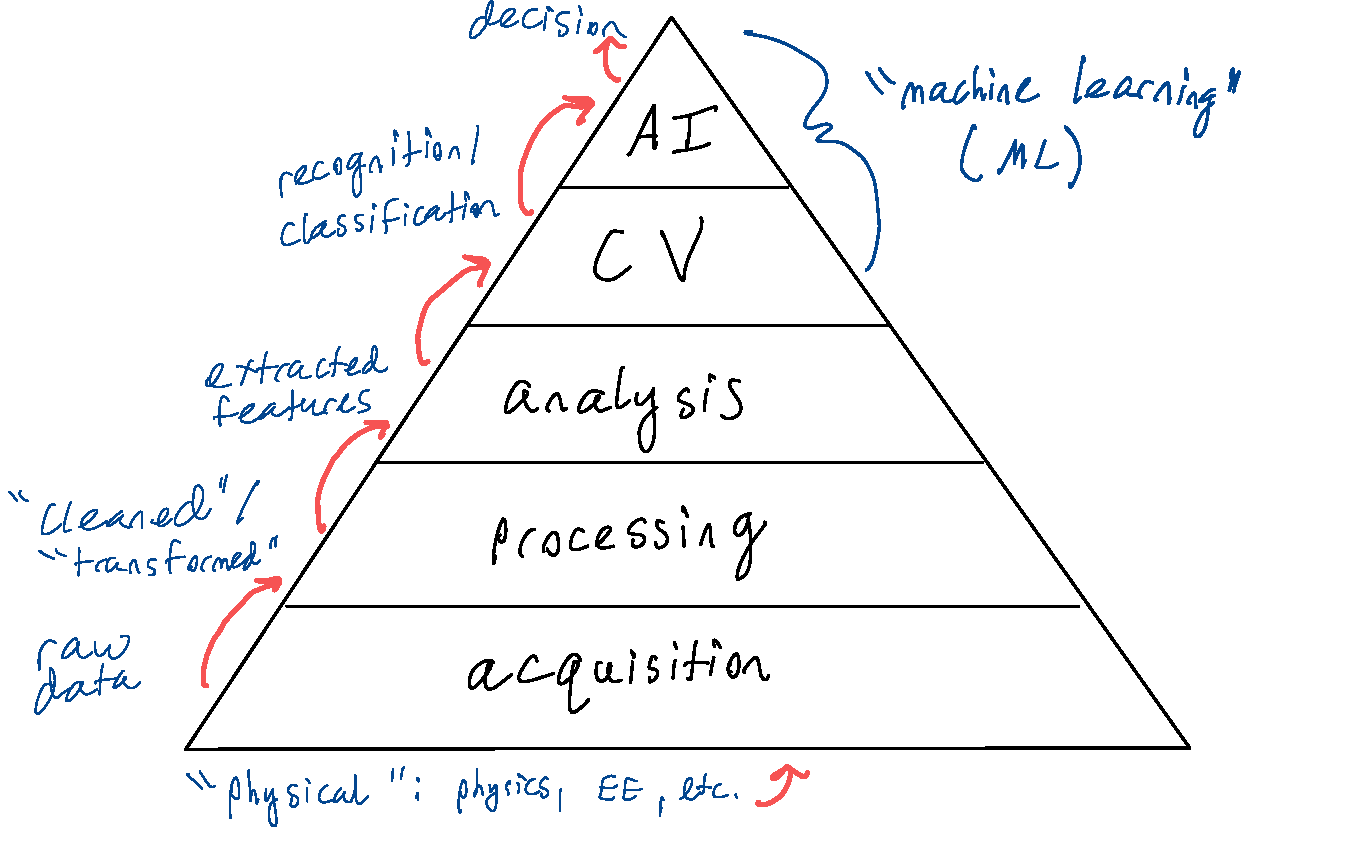
\includegraphics[width=\textwidth]{figures/lecture01/data-processing-pyramid.pdf}
    \caption{Caption}
    \label{fig:data prcessing hierarchy}
\end{figure}



\section{Intro to Sampling and Quantization}

\section{Sampling}

\begin{figure}
    \centering
    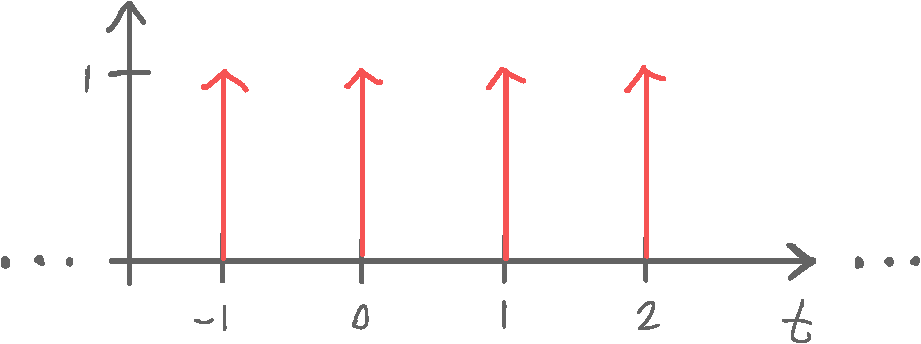
\includegraphics[width=\textwidth]{figures/lecture01/sampling-function.pdf}
    \caption{Caption}
    \label{fig:sampling function}
\end{figure}

\begin{figure}
    \centering
    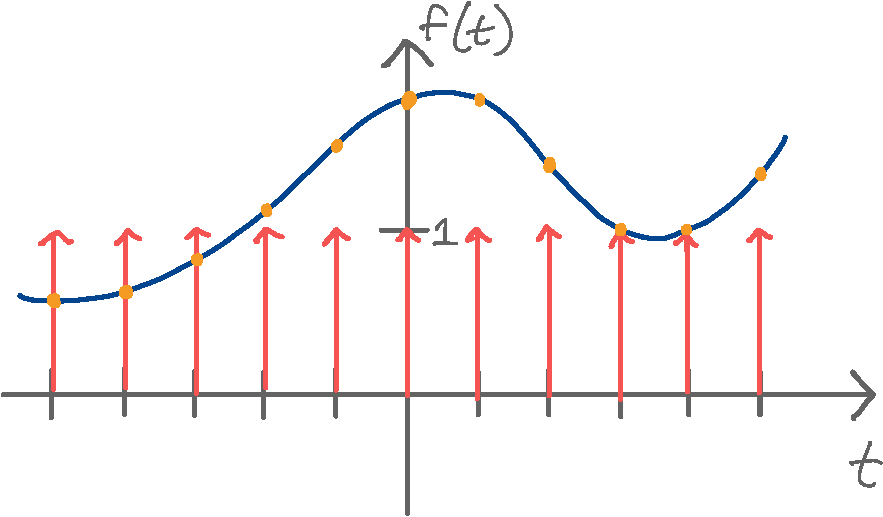
\includegraphics[width=\textwidth]{figures/lecture01/sampling-an-arbitrary-function.pdf}
    \caption{Caption}
    \label{fig:sampling an arbitary function}
\end{figure}


\section{Quantization}


\begin{figure}
    \centering
    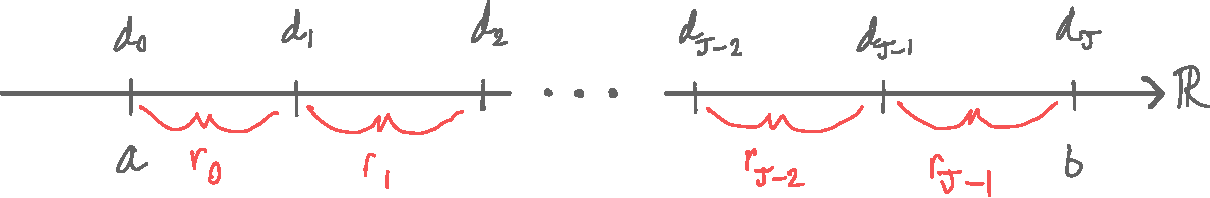
\includegraphics[width=\textwidth]{figures/lecture01/quantization-ranges.pdf}
    \caption{Caption}
    \label{fig:sampling function}
\end{figure}

\begin{figure}
    \centering
    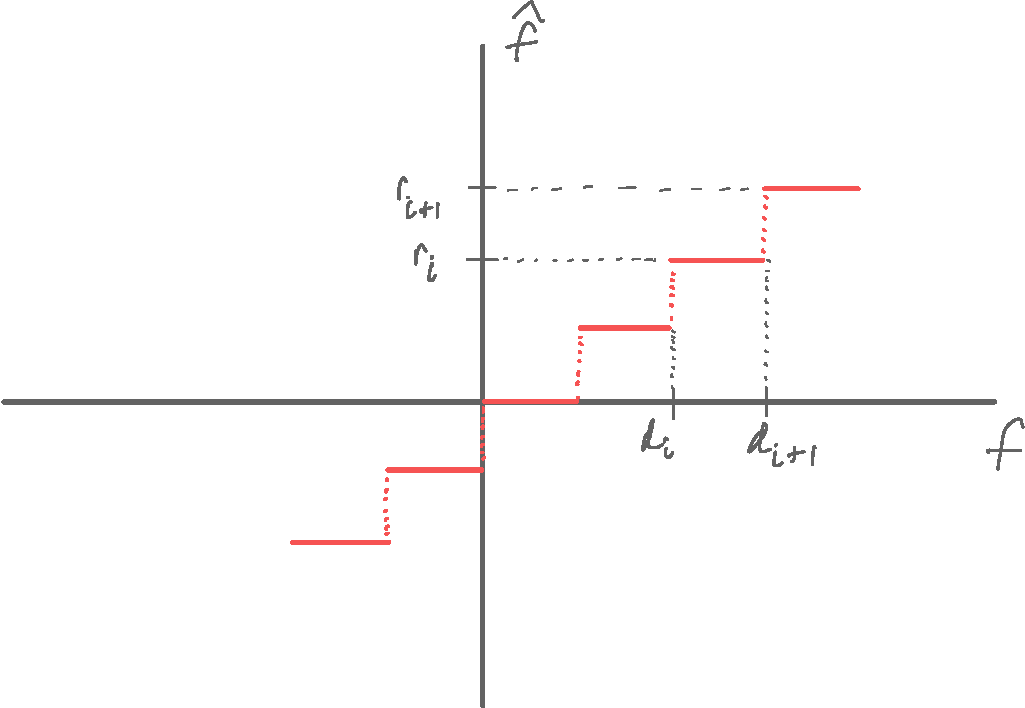
\includegraphics[width=\textwidth]{figures/lecture01/quantization-transfer-function.pdf}
    \caption{Caption}
    \label{fig:sampling an arbitary function}
\end{figure}


\subsection{Quantization error}


\section{Exercises}

\lstinputlisting[language=Matlab]{listings/lecture01/audiotest.m}





%%%%%%%%%%%%%%%%%%%%%%%%%%%%%%%%%%%%%%%%%%%%%%%%%%%%%%%%%%%%%%%%%%%%%%%%%%%%%%%%%%%%%%%%%%%%%%%%%%%%%%%%%%%%%%%%%%%%%%%%%%%%%%%%%%%%
\bibliographystyle{ieeetr}
\bibliography{references}

\end{document}